

\chapter{Joint Executions}

\label{ch:jointexec}

This chapter constructs a new representation for the actions to be
performed by a team of agents during the cooperative execution of
a shared task. Dubbed \emph{joint executions}, they are partially-ordered
branching sequences of actions that allow independent actions to be
performed independently, while using each agent's local view to ensure
that synchronisation is always possible when required.

The fundamental unit of reasoning in the situation calculus, and the
output of the standard Golog execution planning process, is the \emph{situation}:
a complete, ordered sequence of all actions that are to be performed.
This is suboptimal for representing plans in an asyncrhonous multi-agent
setting in three ways:

\begin{itemize}
\item it does not permit branching depending on information obtained at
run-time 
\item it enforces a strict execution order on actions that are potentially
independent, requiring inter-agent syncrhonisation when it is not
actually necessary 
\item it demands a strict execution order on actions that may be hidden
from some agents, demanding inter-agent synchronisation that is not
actually possible 
\end{itemize}
As we have demonstrated in Chapter \ref{ch:mindigolog}, restricting
the domain to be synchronous and completely known lets the agents
make effective use of raw situation terms for planning. But moving
to asynchronous domains with incomplete knowledge requires a more
powerful structure for representing the actions to be performed.

To build such a structure, we take inspiration from a model of concurrent
computation known as \emph{prime event} \emph{structures}, which are
partially-ordered branching sequences of events. A \emph{joint execution}
is defined as a particular kind of prime event structure that is rich
enough to capture the concurrent execution of independent actions,
and can branch on the sensing results of actions. They can also be
reasoned about using standard regression techniques, and built up
one action at a time in much the same way as ordinary situation terms.
Using our explicit account of the local \emph{view} of each agent
from Chapter \ref{ch:observations}, we identify several restrictions
on a joint execution that ensure it is feasible to execute in the
real world.

Joint executions thus allow us to capture the actions that a team
of agents are to perform in service of some shared task, without requiring
constant synchronization between the agents, and without assuming
that agents know all the actions that have been performed, while utilizing
the existing reasoning methods and planning machinery of the situation
calculus. This is a significant increase in expressiveness over existing
approaches to planning for multi-agent teams. To demonstrate the utility
of the approach, we extend our MIndiGolog interpreter from Chapter
\ref{ch:mindigolog} to show how a team of agents can cooperate to
plan and perform the execution of a shared program in an asynchronous,
partially observable domain.

The chapter proceeds as follows: TODO.


\section{Background\label{sec:JointExec:Background}}

The above discussion highlighted three desirable properties of a plan
representation formalism intended for use in rich multi-agent domains:
it must be \emph{partially-ordered}, \emph{branching}, and \emph{feasible}.
While each of these aspects have been studied in isolation in the
situation calculus, our work is the first to combine them into a single
formalism suitable for a multi-agent setting.


\subsection{Partial Orders}

There has been little work on partial-order planning in the situation
calculus, most likely because the use of situations heavily biases
the reasoning machinery towards totally-ordered sequences of actions.
While \citet{son00htn_golog} allow the programmer to specify partial-orders
on actions by adding operators to the Golog language, the actual plans
produced by their system are still raw situation terms. One exception
is \citep{plaisted97sc_aspect}, which extends the situation calculus
with explicit {}``aspects'' and allows partial ordering between
actions that affect different aspects of the world state. By contrast,
we seek to leverage the existing meta-theory of the standard situation
calculus.

Partial-order planning is the mainstay of the closely-related event
calculus formalism. Here each action is specified to happen at a specific
time, and the constraints on relative occurrence times of actions
determine a partial ordering. \citet{Shanahan97ec_planning} has shown
that abductive theorem proving in the event calculate generates partially-ordered
plans, and the mechanics of the theorem prover naturally mirror various
concepts from partial-order planning literature, such as threats and
links \citep{peot92conditional_nonlinear}.

The close similarities between the situation and event calculi are
well understood, as are the advantages of the event calculus when
it comes to working with partially-ordered action sequences \citep{belleghem97sitcalc_evtcalc}.
Indeed, it is possible to implement a Golog interpreter on top of
the event calculus that naturally generates partially-ordered plans
\citep{pereira04ec_golog}. Perhaps we should simply adopt a formalism
such like the event calculus that is naturally partially-ordered,
rather than trying to construct partial orders on top of the naturally
sequential situation calculus?

While having a partial-order representation is important, it is not
the complete picture. We don't want the agents to have to synchronise
their actions unnecessarily, but we also need to ensure the converse:
that when an explicit ordering between actions is necessary, the required
synchronisation is actually possible. It is not clear how techniques
such as \citep{pereira04ec_golog} would extend to the asynchronous
multi-agent case.

As we shall see, the formalism we develop in this chapter enables
these dual requirements - that some actions don't need to be ordered,
while other actions must not be ordered - to be captured in the situation
calculus in quite an elegant way.


\subsection{Branching}

Several single-agent formalisms based on the situation calculus have
introduced some form of branching into the structures returned by
the planner, including the conditional action trees of of sGolog \citep{lakemeyer99golog_cats}
and the branching IndiGolog plans of \citep{giacomo04sem_delib_indigolog}.
These structures typically branch based on the truth or falsehood
of test conditions included in the program, rather than directly on
the sensing results returned by an action. For example, the definition
of conditional action trees in \citep{lakemeyer99golog_cats} includes
the following branching case:\[
c=[\phi,c_{1},c_{2}]\]


This instructs the agent to execute the sub-tree $c_{1}$ if $\phi$
is true and the sub-tree $c_{2}$ if $\phi$ is false. While this
works well for a single agent, it is not clear how to extend it to
cooperative execution in a multi-agent setting, where some members
of the team may not know whether or not $\phi$ holds.


\subsection{Feasibility\label{sec:JointExec:BG:Feasibility}}

To allow an agent to execute a plan that depends on information collected
at run-time, it is not sufficient to simply introduce branching into
the plan representation formalism. One must also ensure that, at execution
time, the agent will always \emph{know} which branch of the plan to
take. For example, suppose this simple branching plan will provably
achieve a goal:\[
\mathbf{if}\,\phi\,\mathbf{then}\, action_{1}\,\mathbf{else\,}\, action_{2}\]


The agent can only execute this program if it knows whether or not
$\phi$ holds; otherwise, although one of the branches is guaranteed
to achieve the goal, the agent does not know which branch to take.
Feasibility is typically guaranteed by including sensing actions to
ensure that the test conditions are known:\[
sense_{\phi}\,;\,\mathbf{if}\,\phi\,\mathbf{then}\, action_{1}\,\mathbf{else\,}\, action_{2}\]


This requirement that an agent {}``knows how'' to execute a plan
is formalised by various notions of \emph{epistemic feasibility},
including those of \citep{levesque98what_robots_can_do,levesque00knowing_how,Lesperance01epi_feas_casl,giacomo04sem_delib_indigolog,baier06programs_that_sense}.

One approach to ensuring feasibility, embodied by \citep{levesque00knowing_how,giacomo04sem_delib_indigolog,baier06programs_that_sense},
is to represent plans by arbitrary programs formulated in a control
language such as Golog. One then semantically characterises the class
of epistemically feasible programs, using direct assertions about
the knowledge of each agent at each stage of execution. While this
allows for potentially very rich, very succinct plans, it is not clear
how to systematically generate an epistmically feasible plan using
such a general characterisation.

Another approach, advocated by \citep{levesque96what_is_planning,levesque98what_robots_can_do}
and used in the implementation section of \citep{giacomo04sem_delib_indigolog},
is to restrict the structure of plans so that they are always epistemically
feasible. For example, the {}``robot programs'' of \citep{levesque98what_robots_can_do}
are restricted to simple operators such as:\begin{gather*}
action\\
seq(\delta_{1},\delta_{2})\\
branch(action,\delta_{1},\delta_{2})\\
loop(branch(action,\delta,exit))\end{gather*}


These programs do not contain test conditions, but rather branch directly
on the (binary) sensing results returned from each action. There is
therefore no potential for confusion when executing such programs;
they are essentially equivalent to a kind of finite automaton that
can be executed reactively. Nevertheless, \citet{levesque98what_robots_can_do}
show that these programs are universal, in the sense that any achievable
goal can be achieved by suitable a robot program. We are not aware
of any work extending this approach to represent programs to be exeuted
cooperatively by a team of agents.

These existing notions of epistemic feasibility can be characterised
as \emph{knowing what}. At each stage of execution, each agent must
know what its next action is. In synchronous domains with public actions,
as typically studied in the situation calculus, this is sufficient
to ensure the feasibility of executing a plan.

In asynchronous domains it is not enough for an agent to know \emph{what}
its next action is; it must also know \emph{when} that action should
be performed. For example, suppose that the following simple plan
provably achieves a goal:\[
action_{1}(agt_{1})\,;\, action_{2}(agt_{2})\]


In a synchrononous domain this plan can be executed directly. But
suppose the domain is asynchronous, and $agt_{2}$ is unable to observe
the occurrence of $action_{1}$. Since $agt_{2}$ has no way of knowing
whether or not $action_{1}$ has been performed, it will not know
when to perform $action_{2}$ and the plan cannot be executed.

In this chapter we ensure plan feasibility by restricting the structure
used to represent plans, in an approach similar to \citep{levesque98what_robots_can_do}
but without looping constructs. We use the explicit account of each
agent's local view developed in the previous chapter to ensure that
each agent will always have enough information to determine what action
to perform next, and when to perform it.


\subsection{Event Structures}

To tackle cooperative execution in a multi-agent setting, we have
adopted a model of concurrent computation known as \emph{event structures}
\citep{npw79event_structures}. The particular variant we are interested
in are \emph{prime event structures}, canonically defined as a four-tuple
as follows.

\begin{defnL}
[{Prime~Event~Structure}] A prime event structure is a
four-tuple $(\mathcal{V},\gamma,\prec,\oplus)$ where: $\mathcal{V}$
is a set of events; $\gamma$ is a function assigning a label to each
event; $\prec$ is the precedence relation, a strict partial order
on events; $\oplus$ is the conflict relation, a binary symmetric
relation indicating events that are mutually exclusive. 
\end{defnL}
The labels assigned by $\gamma$ represent the actions that may occur
in the world, and each event represents a potential occurrence of
an action. Which events can occur at each stage of execution is determined
by $\prec$ and $\oplus$. A \emph{configuration} is a sequence of
events consistent with $\prec$ in which no pair of events conflict.
Each configuration represents a potential partial run of execution
of the system.

As it can be cumbersome to specify $\prec$ and $\oplus$ in their
entirety, we will frequently give only the direct \emph{enablers}
and \emph{alternatives} for each event, denoted by $ens(i)$ and $alts(i)$
respectively. Construction of $(\prec,\oplus)$ from $(ens,alts)$
is a straightforward transitive closure. Formally, the enablers and
alternatives of an event are the largest sets satisfying:\begin{gather*}
j\in ens(i)\equiv j\prec i\,\wedge\,\forall k\in ens(i):\,\neg(j\prec k)\\
j\in alts(i)\equiv j\#i\,\wedge\,\forall k\in ens(i):\,\neg(j\oplus k)\end{gather*}


Considered in this way, event structures form a directed acyclic graph
of the events that could occur during execution of the system. As
shown in \citep{pratt91modeling_conc_with_geom}, these structures
are a canonical representation of a variety of formalisms for representing
concurrent execution, and it is straightforward to convert them into
a kind of finite automaton for efficient execution.


\section{Joint Executions\label{sec:JointExec:JEs}}

This section defines the precise structure of a joint execution, first
using a high-level intuitive description, and then formally as a set
of axioms to be included in the theory of action $\Dt$. Since we
intend for agents to synthesise joint executions as the output of
a planning process, they must exist as concrete terms in the logic.


\subsection{Intuitions}

We define a \emph{joint execution} as a special kind of prime event
structure as follows:

\begin{defnL}
[{Joint~Execution}] A joint execution is a tuple $(\mathcal{A},\mathcal{O},ens,alts,\gamma,<)$
where: action events $\mathcal{A}$ represent actions to be performed;
outcome events $\mathcal{O}$ represent possible outcomes of actions;
$(\mathcal{A}\cup\mathcal{O},ens,alts,\gamma)$ forms a prime event
structure with precedence relation $\prec$; $<$ is a total order
on events that is consistent with $\prec$. 
\end{defnL}
A joint execution contains two disjoint sets of events: \emph{action}
events $\mathcal{A}$ representing the actions to be performed, and
\emph{outcome} events $\mathcal{O}$ representing the possible outcomes
of each action. For each action event $i\in\mathcal{A}$, its enablers
$ens(i)$ is a set of outcome events, its alternatives $alts(i)$
is empty, and its label $\gamma(i)$ is the action to be performed.
For each outcome event $i\in\mathcal{O}$, $ens(i)$ is a single action
event for which it is a possible outcome, $alts(i)$ is the set of
all other outcome events $j$ such that $ens(j)=ens(i)$, and $\gamma(i)$
is an outcome as produced by the $Out(a,s)$ function for the action
$\gamma(ens(i))$.

Each action event thus represents a single action to be performed,
which enables several alternative outcome events corresponding to
the potential results returned by that action; since an action can
only produce one outcome, the enabled outcome events are all mutually
conflicting. Each of these outcome events can then enable further
action events, and so forth. A simple example of a joint execution
is shown in Figure \ref{fig:example-je}. TODO: redo this diagram,
and describe it.

%
\begin{figure}
\framebox{%
\begin{minipage}[t][1\totalheight]{1\columnwidth}%
\textsf{\textbf{\tiny 
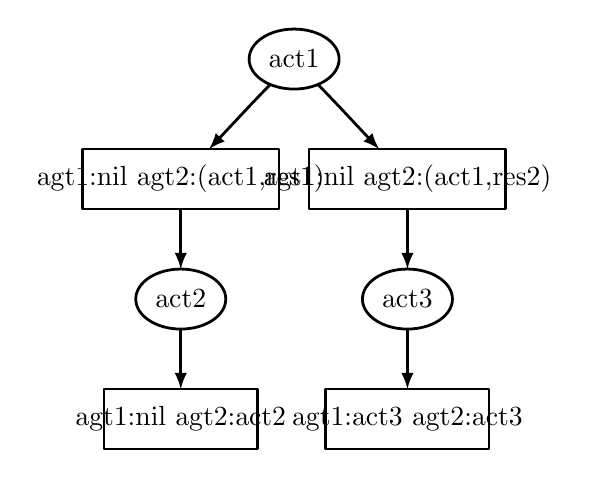
\begin{tikzpicture}[>=latex,join=bevel,scale=0.60]
  \pgfsetlinewidth{1bp}
%
\pgfsetcolor{black}
  % Edge: n1 -> n2
  \draw [->] (113bp,219bp) .. controls (104bp,210bp) and (93bp,198bp)  .. (76bp,180bp);
  % Edge: n1 -> n3
  \draw [->] (141bp,219bp) .. controls (150bp,210bp) and (161bp,198bp)  .. (178bp,180bp);
  % Edge: n4 -> n5
  \draw [->] (59bp,72bp) .. controls (59bp,64bp) and (59bp,55bp)  .. (59bp,36bp);
  % Edge: n6 -> n7
  \draw [->] (195bp,72bp) .. controls (195bp,64bp) and (195bp,55bp)  .. (195bp,36bp);
  % Edge: n2 -> n4
  \draw [->] (59bp,144bp) .. controls (59bp,136bp) and (59bp,127bp)  .. (59bp,108bp);
  % Edge: n3 -> n6
  \draw [->] (195bp,144bp) .. controls (195bp,136bp) and (195bp,127bp)  .. (195bp,108bp);
  % Node: n1
\begin{scope}
  \pgfsetstrokecolor{black}
  \draw (127bp,234bp) ellipse (27bp and 18bp);
  \draw (127bp,234bp) node {act1};
\end{scope}
  % Node: n2
\begin{scope}
  \pgfsetstrokecolor{black}
  \draw (118bp,180bp) -- (0bp,180bp) -- (0bp,144bp) -- (118bp,144bp) -- cycle;
  \draw (59bp,162bp) node {agt1:nil agt2:(act1,res1)};
\end{scope}
  % Node: n3
\begin{scope}
  \pgfsetstrokecolor{black}
  \draw (254bp,180bp) -- (136bp,180bp) -- (136bp,144bp) -- (254bp,144bp) -- cycle;
  \draw (195bp,162bp) node {agt1:nil agt2:(act1,res2)};
\end{scope}
  % Node: n4
\begin{scope}
  \pgfsetstrokecolor{black}
  \draw (59bp,90bp) ellipse (27bp and 18bp);
  \draw (59bp,90bp) node {act2};
\end{scope}
  % Node: n5
\begin{scope}
  \pgfsetstrokecolor{black}
  \draw (105bp,36bp) -- (13bp,36bp) -- (13bp,0bp) -- (105bp,0bp) -- cycle;
  \draw (59bp,18bp) node {agt1:nil agt2:act2};
\end{scope}
  % Node: n6
\begin{scope}
  \pgfsetstrokecolor{black}
  \draw (195bp,90bp) ellipse (27bp and 18bp);
  \draw (195bp,90bp) node {act3};
\end{scope}
  % Node: n7
\begin{scope}
  \pgfsetstrokecolor{black}
  \draw (244bp,36bp) -- (146bp,36bp) -- (146bp,0bp) -- (244bp,0bp) -- cycle;
  \draw (195bp,18bp) node {agt1:act3 agt2:act3};
\end{scope}
%
\end{tikzpicture}

}}{\tiny {} }%
\end{minipage}}

\caption{ A simple joint execution. Elliptical nodes are action events, box
nodes are outcome events. }


\label{fig:example-je} 
\end{figure}


Recall that a \emph{configuration} is a partial run of execution of
the prime event structure. Clearly any configuration ending in an
outcome event corresponds to a unique situation term and also a unique
history term, as it is a set of alternating actions and their outcomes.

We will call a set of unordered, non-conflicting outcome events an
\emph{outcome set} and denote it $os$. A \emph{branch} is a special
case of an outcome set where every event is either in the branch,
conflicts with something in the branch, or precedes something in the
branch: \[
\forall i\in\mathcal{O}:\,\, i\in b\,\equiv\,\neg(\exists j\in b:\,\, i\oplus j\,\vee\, i\prec j)\]


A branch thus represents potential \emph{terminating} runs of the
execution. TODO: demonstrate branches in the example JE.

The \emph{histories} of an outcome set is the set of all configurations
that contain all elements of $os$, and end in an event from $os$.
By these definitions, the union of histories of all branches gives
the set of all histories that could be produced by performing the
joint execution.

A joint execution has one additional component over a standard prime
event structure: a \emph{total} order on events $<$ that is consistent
with the partial order $\prec$ induced by the enabling relation.
We call this the \emph{canonical ordering}, and it allows any branch
to be unambiguosly translated into a \emph{canonical history}. When
we come to use joint executions for planning, we will use the canonical
history to avoid having to reason about all the (potentially exponentially-many)
histories of each branch. The canonical ordering is determined by
the order of insertion of events into the structure.


\subsection{Formalities}

We introduce new sorts \noun{Event }and \noun{JointExec} to $\Lsit$,
and will collect the axioms defining joint executions in a separate
axiom set $\Dt_{je}$. Events are opaque identifiers with which a
joint execution associates a label, a set of enablers, and a set of
alternatives. For simplicity we will identify events with the integers,
although our definitions require only the successor function and ordering
relation. Labels are either \noun{Action} or \noun{Outcome} terms.


\subsubsection{Structural Axioms}

A joint execution consists of:

\begin{itemize}
\item a set of \emph{events}, which are integer ids 
\item a mapping from each event to a \emph{label}, which is either an action
or an outcome 
\item a mapping from each event to its \emph{enablers}, which is a set of
lower-numbered events 
\item a mapping from each event to its \emph{alternatives}, which is a set
of events 
\end{itemize}
As a base case, we have the empty joint execution as follows:

\[
JExec_{0}\,\isdef\, jexec(\{\},\{\},\{\},\{\})\]


The following four functions access the mappings contained in a joint
execution:\begin{gather*}
events(je)=es\,\equiv\exists ls,ns,as:\, je=jexec(es,ls,ns,as)\\
lblmap(je)=ls\,\equiv\exists es,ns,as:\, je=jexec(es,ls,ns,as)\\
ensmap(je)=ns\,\equiv\exists es,ls,as:\, je=jexec(es,ls,ns,as)\\
altsmap(je)=as\,\equiv\exists es,ls,ns:\, je=jexec(es,ls,ns,as)\end{gather*}


We also define the following shortcut accessors to get the value from
each mapping for a particular event $i$:\begin{gather*}
lbl(je,i,l)\equiv i\#l\in lblmap(je)\\
ens(je,i,ns)\equiv i\#ns\in ensmap(je)\\
alts(je,i,as)\equiv i\#as\in altsmap(je)\end{gather*}


For notational convenience we will often write these as functions,
but this should be understood as an abbreviation since not every joint
execution will contain every event. For example:\[
ens(je,i)=ns\,\isdef\,\exists ns':\, ens(je,i,ns')\wedge ns'=ns\]
 Like standard situation terms, joint executions are built up by progressively
inserting new events into an existing joint execution. First, we have
a function to get the id of the next event:\[
NextEvent(je)=max(\{0\}\cup events(je))+1\]


To add to a joint execution, we must specify the predecessor joint
execution, the label for the new event, and its set of enablers. The
set of alternatives for the new event is determined automatically
based on the required structure of the joint execution -- action events
have no alternatives, while outcome events must have as their alternatives
every other outcome event enabled by the same action.

The following predicate specifies the conditions under which such
an insertion forms a valid joint execution, according to the intuitions
discussed above:\begin{gather*}
Insert(je,lb,ns,,je')\equiv\exists i:\, NextEvent(je)=i\\
\wedge\, events(je')=events(je)\cup\{i\}\\
\wedge\, lblmap(je')=lblmap(je)\cup\{i\#lb\}\\
\wedge\, ensmap(je')=ensmap(je)\cup\{i\#ns\}\\
\wedge\left(InsertOut(je,i,lb,ns,je')\vee InsertAct(je,i,lb,ns,je')\right)\end{gather*}


Note that this is not a function, since an invalid set of enablers
could cause it to be false. Outcome events must be enabled by a single
action event, and the alternatives must be updated for all other outcome
events associated with that action:\begin{gather*}
InsertOut(je,i,lb,ns,je')\equiv\,\,\,\,\,\, IsOutcome(lb)\\
\wedge\exists j,a:\, ns=\{j\}\wedge lbl(je,j,a)\wedge IsAction(a)\\
\wedge\left(\exists allAlts:\,\forall k:\, k\in allAlts\equiv ens(je',k,\{j\})\right)\\
\wedge\forall k:\,\left[k\not\in events(je')\,\rightarrow\,\neg\exists as:\, alts(je',k,as)\right]\\
\wedge\left[ens(je',k,\{j\})\rightarrow alts(je',k,allAlts)\right]\\
\wedge\left[\neg ens(je',k,\{j\})\rightarrow\exists as:\, alts(je,k,as)\wedge alts(je',k,as)\right]\end{gather*}


Action events must be enabled by a set of outcome events and cannot
have any alternatives:\begin{gather*}
InsertAct(je,i,lb,ns,je')\equiv\,\,\,\,\,\, IsAction(lb)\\
\wedge\forall j\in ns:\,\exists lb':\, lbl(je,j,lb')\wedge IsOutcome(lb')\\
\wedge altsmap(je')=altsmap(je)\cup\{i\#\{\}\}\end{gather*}


Finally, we need a second-order induction axiom stating that the only
joint executions are those that can be constructed in this way. This
is entirely analogous to the axiom for situation terms:\begin{multline*}
\forall P:\,\left[P(JExec_{0})\wedge\forall je,je',lb,ns:\, P(je)\wedge Insert(je,lb,ns,je')\rightarrow P(je')\right]\\
\rightarrow\forall je:\, P(je)\end{multline*}


These definitions enforece the basic structure of a joint execution,
but do not constrain it to be something that could be executed in
the world -- for example, outcomes can be enabled by actions that
will never actually produce that outcome. Like situation terms, we
focus first on getting the appropriate structure, and then specify
additional conditions that joint executions must satisify in order
to be legal in the real world.

Note that we have placed an important restriction on the ordering
of events -- if $i<j$ according to the total ordering over the integers,
then it is not possible for $i$ to be enabled by $j$. This does
not result in a lack of expressiveness, since if we want $i$ to be
enabled by $j$, then $j$ must not be enabled by $i$ and we can
simply give $j$ the lower event number.

Now, let us define the \emph{preceeds} and \emph{conflicts} relations
in terms of enablers and alternatives. We will write these as binary
infix operators $\prec_{je}$ and $\oplus_{je}$. The precedence relation
is defined as a transitive closure over enablers:\begin{multline*}
\forall P,i,j:\left[\left(i\in ens(je,j)\,\rightarrow P(i,j)\right)\,\wedge\,\left(\forall k:\, P(i,k)\wedge k\in ens(je,j)\,\rightarrow\, P(i,j)\right)\right]\\
\rightarrow\left(P(i,j)\rightarrow i\prec_{je}j\right)\end{multline*}


The conflict relation is defined so that $i\oplus j$ if they have
altnerative predecessors:\begin{multline*}
\forall P,i,j:\,\left[\left(i\in alts(je,j)\,\rightarrow P(i,j)\right)\right.\\
\left.\wedge\,\left(\forall i',j':\, P(i',j')\wedge i'\preceq_{je}i\wedge j'\preceq_{je}j\,\rightarrow\, P(i,j)\right)\right]\\
\rightarrow\left(P(i,j)\rightarrow i\oplus_{je}j\right)\end{multline*}


These axioms suffice to give an account of joint executions as prime
event structures as defined in \citep{npw79event_structures}.


\subsubsection{Additional Notions}

We also require some additional definitions and notation that is not
typically found in the literature on prime event structures, in order
to related joint executions back to the existing concepts of the situation
calculus.

An \emph{outcome set} is a set of unordered non-conflicting outcome
events; that is, a set of events satisfying:\begin{multline*}
OutcomeSet(je,os)\,\equiv\,\forall i,j\in os:\, IsOutcome(lbl(je,i)\\
\wedge IsOutcome(lbl(je,j)\\
\wedge\,\neg(i\oplus_{je}j)\,\wedge\, i\not\prec_{je}j\,\wedge\, j\not\prec_{je}\, j\end{multline*}


An outcome set identifies a family of potential partial runs of the
execution. We can generate these histories by recursively selecting
an event that does not conflict with anything in $os$ and is enabled
given what we have performed so far:

TODO

An outcome set $os$ \emph{covers} a set \emph{$os'$,} denoted by
$os\sqsubseteq_{je}os'$, if every event in $os$ is either also in
$os'$, or precedes something in $os'$. Every history in $hists(os')$
will have a prefix in $hists(os)$. This defines a partial ordering
on outcome sets:\[
os\sqsubseteq_{je}os'\,\equiv\,\forall i\in os:\,\,\exists i'\in os':\,\, i\preceq_{je}i'\]


A \emph{branch}, denoted $b$, is a special case of an outcome set
that meets the following additional requirement:\[
Branch(je,b)\,\equiv\,\forall i\in events(je):\, i\in b\,\equiv\,\neg(\exists i'\in b:\,\, i\oplus i'\,\vee\, i\prec i')\]



\subsection{Feasible Joint Executions}

We now impose two restrictions on joint executions to ensure that
they are \emph{feasible} -- that the agents will actually be able
to perform them in the world.

The first restriction corresponds to the idea of \emph{knowing when}
to perform an action. If an action event $i$ is enabled by an outcome
event $j$ produced by another agent, the agent performing $i$ must
be able to observe the occurrence of $j$. Otherwise, it has no way
of synchronizing its actions with those of its teammate. Let $actor(i)$
be the agent responsible for performing an action event $i$, then
we require that:\[
\forall i,j\in events(je):\, IsAction(lbl(je,i))\,\wedge j\in ens(je,i)\rightarrow\, lbl(je,j)[actor(je,i)]\neq\{\}\]


The second restriction corresponds to the idea of \emph{knowing what}
action to perform. For a given event $i$, define the enabling views
of $i$ are all views in in which the agent responsible for $i$ could
be required to execute it:\[
EnablingView(je,i,v)\equiv\exists agt,h:\, actor(je,i)=agt\wedge Hist(je,ens(je,i),h)\wedge View(agt,h)=v\]


This definition gives all the possible views of $agt$ in which event
$i$ is enabled, and so the agent is required to perform action $lbl(je,i)$.
Since the agent has only a local viewpoint, it is possible that some
other outcome set can produce an identical view. Say that two outcome
sets overlap, denoted $Overlaps(je,agt,os,os')$, if they could produce
an identical local history for a given agent:\[
\exists v:\, EnablingView(je,view(agt,hists(e_{1}))\,\cap\, view(agt,hists(e_{2}))\,\neq\varnothing\]


TODO: formulate this properly

Then the \emph{minimal overlapping set} for $e_{1}$, from the perspective
of $agt$, is the set of all $e_{2}$ satisfying:\begin{multline*}
e_{2}\in minovlp(agt,e_{1})\,\equiv\\
ovlaps(agt,e_{1},e_{2})\wedge\neg\exists e_{3}\left[ovlaps(agt,e_{1},e_{3})\wedge e_{3}\sqsubset e_{2}\right]\end{multline*}


This captures all outcome sets that the agent could potentially confuse
for $e_{1}$. To ensure there is no confusion about whether an action
is enabled, for each $i\in\mathcal{A}$, every $e$ in the minimal
overlapping set of $ens(i)$ for $actor(i)$ must enable an event
$i'$ with identical action $\gamma(i')=\gamma(a)$. Formally:\begin{multline*}
\forall e\in minovlp(actor(i),ens(i)):\,\\
\exists i':\,\gamma(i')=\gamma(i)\,\wedge\, ens(i')=e\end{multline*}
 This ensures that the agent's local information is enough to know
when it should perform an action. While it may not know precisely
which \emph{event} is enabled, it will know enough to determine the
specific \emph{action} that it must perform.

Finally, we say a joint execution is feasible if it meets both these
conditions:\[
Feasible(je)\,\isdef\, KnowsWhat(je)\wedge KnowsWhen(je)\]



\subsection{Legal Joint Executions}

We call a branch of a joint execution \emph{legal} if every history
of that branch corresponds to a legal situation:\[
Legal(je,b)\,\isdef\,\forall h\in Hists(je,b):\,\exists s:\, Legal(s)\wedge History(s)=h\]


In general, the agents will not have enough information to determine
whethe a particular branch is legal, since this would imply that they
already know what sensing results will occur.

We will call a joint execution \emph{legal} if it contains a legal
branch:\[
Legal(je)\,\isdef\,\exists b:\, Branch(je,b)\wedge Legal(b)\]


This definition does not require that we establish \emph{which} branch
is legal, only that we are able to prove that \emph{some} branch must
be legal. It is also permissive, in that is permits redundant branches
that can never be legal. Since these branches will not actually be
taken at execution time, this permissiveness will not affect the agent's
ability to carry out the plan.


\subsection{Planning with Joint Executions}

Finally, we are in a position to plan the cooperative execution of
a shared MIndiGolog program using these structures.


\subsubsection{Offline Planning}

Consider first \emph{offline} planning in the style ConGolog and the
original Golog. The agents need to find a feasible, legal joint execution
such that for every branch, if that branch is legal, then it will
form a legal execution of the program:\begin{multline*}
\Dt\cup\Dt_{mgolog}\cup\Dt_{je}\models\exists je:\, Legal(je)\wedge Feasible(je)\wedge\\
\forall b:\, Branch(je,b)\wedge Legal(je,b)\,\rightarrow\,\left[\forall s:\, Sit(je,b,s)\rightarrow\Do(\delta,S_{0},s)\right]\end{multline*}


This captures a pair of soundness and completeness requirements. For
soundness we require that for every branch of the joint execution,
\emph{if} that branch is legal then it will be a legal execution of
the program. For completeness, we assert that there must be some legal
branch.


\subsubsection{Online Execution}

Capturing online execution is not so straightforward, as it is difficult
to single-step an execution in a partially-observable setting. Consider,
for example, a program whose next step is a sensing action to be performed
by some agent. After executing this step, the performing agent will
know the result of the action, but it cannot necessarily use this
in planning the next step. While the sensing result allow that particular
agent to discard some leaves from the joint execution, it must consider
that other team members may still think those leaves are open. These
team members in turn have their own view of the joint execution...TODO...yadda
yadda common knowledge.

One of the intuitions behind introducing online execution in IndiGolog
was to avoid branching plans, by executing just enough of the program
to gather the necessary sensing results. Following this intuition
in the multi-agent case, the agents should plan just far enough ahead
to ensure thay every team member knows what branch has been taken.\[
Distinguishable(je)\,\isdef\,\forall lf,agt,v:\, View(agt,je,lf)=v\,\rightarrow\neg\exists lf':\, Leaf(je,lf)\wedge View(agt,je,lf)=v\]


In other words, every agent's local view at each leaf is sufficient
to distinguish it from every other leaf.

\begin{multline*}
\Dt\cup\Dt_{mgolog}\cup\Dt_{je}\models\exists je:\, Legal(je)\wedge Feasible(je)\wedge Distinguishable(je)\\
\forall lf:\, Leaf(je,lf)\wedge Legal(je,lf)\,\rightarrow\,\left[\forall s:\, Sit(je,lf,s)\rightarrow Trans^{*}(\delta,S_{0},s)\right]\end{multline*}



\subsubsection{Search}




\subsection{Summary\label{sec:JointExec:Summary}}

In this section we have defined a \emph{joint execution} as a prime
event structure with some additional restrictions. We contend that
such structures are highly suitable for planning the actions to be
performed by a team in service of some shared task, such as executing
a shared Golog program.

On one hand, joint executions are restricted enough to be practical
for such use. Prime event structures are purely reactive (equivalent
to a kind of finite automaton) and can be executed by the agents without
further deliberation. They are restricted to ensure that whenever
an agent is required to perform an action, it is able to determine
this using only its local information. Each branch of execution can
be easily converted into a situation term for the purposes of reasoning,
and can be extended one action at a time.

Joint executions are also significantly more flexible than previous
approaches. They allow independent actions to be performed without
synchronization, in any order. The agents need never know precisely
what actions have been executed, only those that enable them to perform
their next action. Synchronization is automatically achieved when
required by explicitly reasoning about what actions each agent can
observe, rather than requiring that all actions be public.

To demonstrate the utility of these structures, we have implemented
an interpreter for multi-agent ConGolog programs that produces joint
executions as its output. In the next section, we highlight the key
aspects of our implementation and give an example of the output it
produces.


\section{Implementation\label{sec:JointExec:Implementation}}

While these structures so far allow provide a powerful formal account
of execution planning in multi-agent domains, they are not suitable
for an effective implementation. In order to verify that a joint execution
is legal, it is necessary to examine every possible history of every
brach in the execution. Since it is a partially-ordered structure
there is a potentially exponential number of histories for every branch.


\subsection{Canonical Joint Executions}


\subsection{Independent Actions\label{sec:JointExec:IndepActs}}


\subsection{Program Steps}


\subsection{Planning Loop}


\subsection{Distributing the Planning Workload}


\section{Discussion\label{sec:JointExec:Discussion}}

An alternate approach to the problem of partial observability is the
language TeamGolog developed in \citep{farinelli07team_golog}, where
agents explicitly synchronize through communication and a shared state.
By contrast, our approach constructs synchronization implicitly by
reasoning about the actions that can be observed by each agent. This
has the advantage of requiring no changes to the form or semantics
of the agents' control program, but the disadvantage that joint execution
construction may fail if too many actions are unobservable. It would
be interesting to combine these approaches by automatically incorporating
explicit communication when implicit synchronization is not possible.

There is, of course, an extensive body of work on partial-order planning
in the context of goal-based planning. Unsurprisingly, the joint execution
structure we develop here has deep similarities to the structures
used in conditional partial-order planners such as \citep{peot92conditional_nonlinear}.
It is, however, intentionally specific to the situation calculus.
We make no use of many concepts common in partial-order goal-based
planning (causal links, threats, conflicts, etc) because we do not
deal explicitly with goals, but with steps generated by an underlying
transition semantics. Our approach can be considered roughly equivalent
to \emph{deordering} of a totally-ordered plan as described in \citep{backstrom99reordering},
except performed during plan construction rather than as a post-processing
step.

loops: \citep{levesque96what_is_planning,levesque05planning_with_loops}

can't represent actions that {*}need{*} to be performed concurrently
- but should be a trivial addition.

don't use explicit mental attitiudes, mutual beliefs etc. JE's more
akin to recpies in SharedPlans. Assume agents all have the common
goal of executing the given shared program. But it could be used as
part of larger system.

